\documentclass{article} 
\usepackage{fancyhdr,geometry,subfig,hyperref,graphicx,psfrag,amsfonts,mathtools,amsmath} 

\title{Mandatory exercise 3 \\
Signal and Image Processing 2012} 
\author{Jens P. Raaby \\
\url{frn617@diku.dk}}

\begin{document} 
\maketitle

\section*{Question 3.1 - Noisy Signals}
Generating a 100 element vector of samples according to a given noise type was relatively easy with Matlab, with the exception of the Salt and Pepper noise which took some time to understand correctly. 

The file noiseGen1D.m contains a function to generate such samples. The histograms of the samples generated are shown in figure \ref{fig:q1}. These and the parameter estimations are generated in the file q1.m.

In general, fitting parameters to a distribution will be more accurate with more samples. Therefore some of the inaccuracy of any estimates can be explained by the relatively small sample size.

\subsection*{Gaussian}
The Gaussian noise is generated using either of the functions randn and normrnd in MATLAB. It is relatively easy to estimate the parameters of the noisy signal, since they are defined:
\[
\mu = mean(sample)
\]
\[
\sigma = \sqrt{variance(sample)}
\]
Using these equations, I estimated the parameters at $\mu = -0.0528$ and $\sigma = 0.4758$.

\subsection*{Gamma}
Gamma noise parameters are slightly more complex to retrieve, but are still based on the mean and variance (equations 5.2-6 and 5.2-7 in Gonzalez \& Woods). With simple algebraic manipulation the terms $a$ and $b$ can be determined from the variance and mean:
%\begin{equation}
%\begin{array}{rl}
\[
a =  \frac {\mu} {\sigma ^2}
\]
\[
b =  \frac { \mu ^2} {\sigma ^2}
\]
%\end{array}
%\end{equation}
I found in practice that this returned some incorrect results (by testing different parameter values and comparing the estimates with those provided by Matlab's built in fitdist function). However for the given parameters (1,1) the error was not so great. I calculated $a=1.0343$ and $b=1.0801$.

\subsection*{Uniform}
In a similar manner to Gamma noise above, I rearranged the equations from Gonzalez and Woods to give:
\begin{equation}
\begin{array}{rl}
b = & \mu + \frac 1 2 {\sqrt{12\sigma ^2}}\\\\
a = & 2 \mu - b
\end{array}
\end{equation}
The results were quite accurate on the test data, giving $a=0.0667$ and $b=2.0825$.


\subsection*{Salt and pepper}
There was a lot of confusion and time wasting about this part of the assignment. Google did not help! 
My understanding of salt and pepper noise after reading more carefully (in particular the lecture slides provided at \url{http://cronos.rutgers.edu/~lrr/dsp\%20design\%20course/lectures/Lecture_IP5_2009.pdf}) is as follows:
The noise contains pepper (with intensity $a$)  with probability $P_a$, and salt (intensity $b$) with probability $P_b$. All other samples take some other value (with probability $1-(P_a + P_b)$). The original probabilities 0.1 and 0.2 made sense - 10\% of the signal should be pepper noise, and 20\% should be salt noise. The updated assignment changed the probabilities so that they sum to 1 (this is unnecessary, and means that the entire signal is noise!). 

Estimating the parameters is relatively easy when visually inspecting the histogram (see figure \ref{fig1:sandp}): there are two peaks at value 0 and 2, where one peak is twice the height of the other.

Calculating the parameters from the samples using the histogram (binned to the same size as the vector of samples) gave the following estimates:
$a = 0.0100$, $b = 1.9900$, $p_a = 0.3800$,$p_b =  0.6200$. These are close to the input parameters.

\subsection*{Using estimation with real images}
If the noise parameters of real images could be estimated using methods such as those I used above, it may be easier to restore the image to a less noisy condition. For example, if the salt and pepper noise parameters are estimated it should be relatively straightforward to replace the offending pixels (those with intensities $a$ and $b$) with the mean of the pixel neighbourhoods.
In the other types of noise, the pattern is more complex and (being stochastic) quite difficult to eliminate completely from inaccurate estimates. I would expect that using an iterative algorithm might be able to help in this instance. Once a basic estimate of noise parameters is known, subtract a m x n copy of the noise from the image (where the image size is m x n). Inspect the noise of the resulting image, and change each parameter in turn while observing the effect. If there is an improvement (reduction), keep adjusting the parameter in the same way until no improvements are observed. This 'gradient descent' approach would not be particularly practical in many cases. According to Gonzalez and Woods, various mean filters are typically used to smooth away noise from images. The order-statistic filters should yield even better results (for example the median filter mentioned in GW section 5.3.2).


\section*{Question 3.2 - Wiener Filtering}

\section*{Question 3.3 - Long exposure blurring}

\section*{Question 3.4 - Restoration}

\begin{figure}

\subfloat[Gaussian samples ($\mu = 0$, $\sigma = 0.5$)]{\label{fig1:gauss}\includegraphics[width=0.5\textwidth]{q1-gaussian.ps}}
\subfloat[Gamma samples ($a = 1$, $b = 1$)]{\label{fig1:gamma}\includegraphics[width=0.5\textwidth]{q1-gamma.ps}}\\
\subfloat[Uniform samples ($a = 0$, $b = 2$)]{\label{fig1:uniform}\includegraphics[width=0.5\textwidth]{q1-uniform.ps}}
\subfloat[Salt \& Pepper samples ($P_0 = 1/3$, $P_2 = 2/3$)]{\label{fig1:sandp}\includegraphics[width=0.5\textwidth]{q1-sandp.ps}}

\caption{Histograms for noise samples}
\label{fig:q1}
\end{figure}
 \end{document}
